\documentclass[a4paper]{article}

% Set for specific document
\def\DOCTITLE{Hardware Shader Screenshots}
\def\DOCAUTHOR{Dan Nixon (120263697)}
\def\DOCDATE{\today}

% Set document attributes
\title{\DOCTITLE}
\author{\DOCAUTHOR}
\date{\DOCDATE}

\usepackage{fullpage}
\usepackage{scrextend}
\usepackage{titlesec}
\usepackage{fancyhdr}

% Handle graphics correctly
\ifx\pdftexversion\undefined
\usepackage{graphicx}
% \usepackage[dvips]{graphicx}
\else
\usepackage[pdftex]{graphicx}
\DeclareGraphicsRule{*}{mps}{*}{}
\fi

% Setup headers and footers
\pagestyle{fancy}
\lhead{}
\chead{\DOCTITLE}
\rhead{}
\rfoot{\DOCDATE}
\cfoot{\thepage}
\lfoot{\DOCAUTHOR}

% New page for each section
\newcommand{\sectionbreak}{\clearpage}

% Set header and footer sizes
\renewcommand{\headrulewidth}{0.4pt}
\renewcommand{\footrulewidth}{0.4pt}
\setlength{\headheight}{15.2pt}
\setlength{\headsep}{15.2pt}

\begin{document}

\begin{figure}[h!]
  \centering
  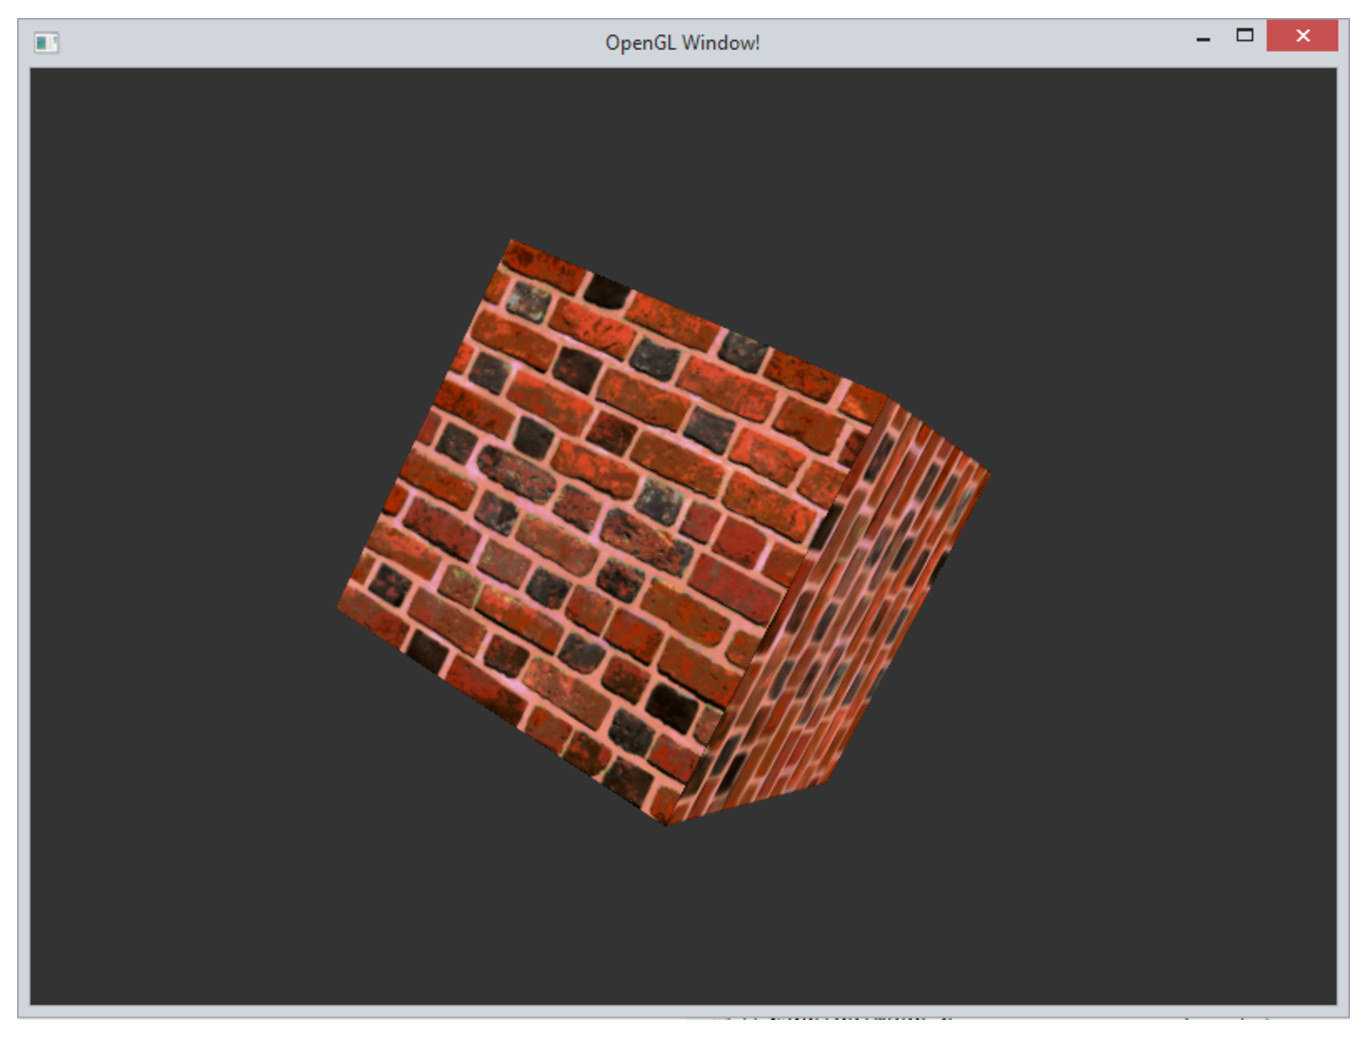
\includegraphics[width=0.50\textwidth]{graphics/screen_1.eps}
  \caption{Fading between two textures}
  \label{fig:screen_1}
\end{figure}

\begin{figure}[h!]
  \centering
  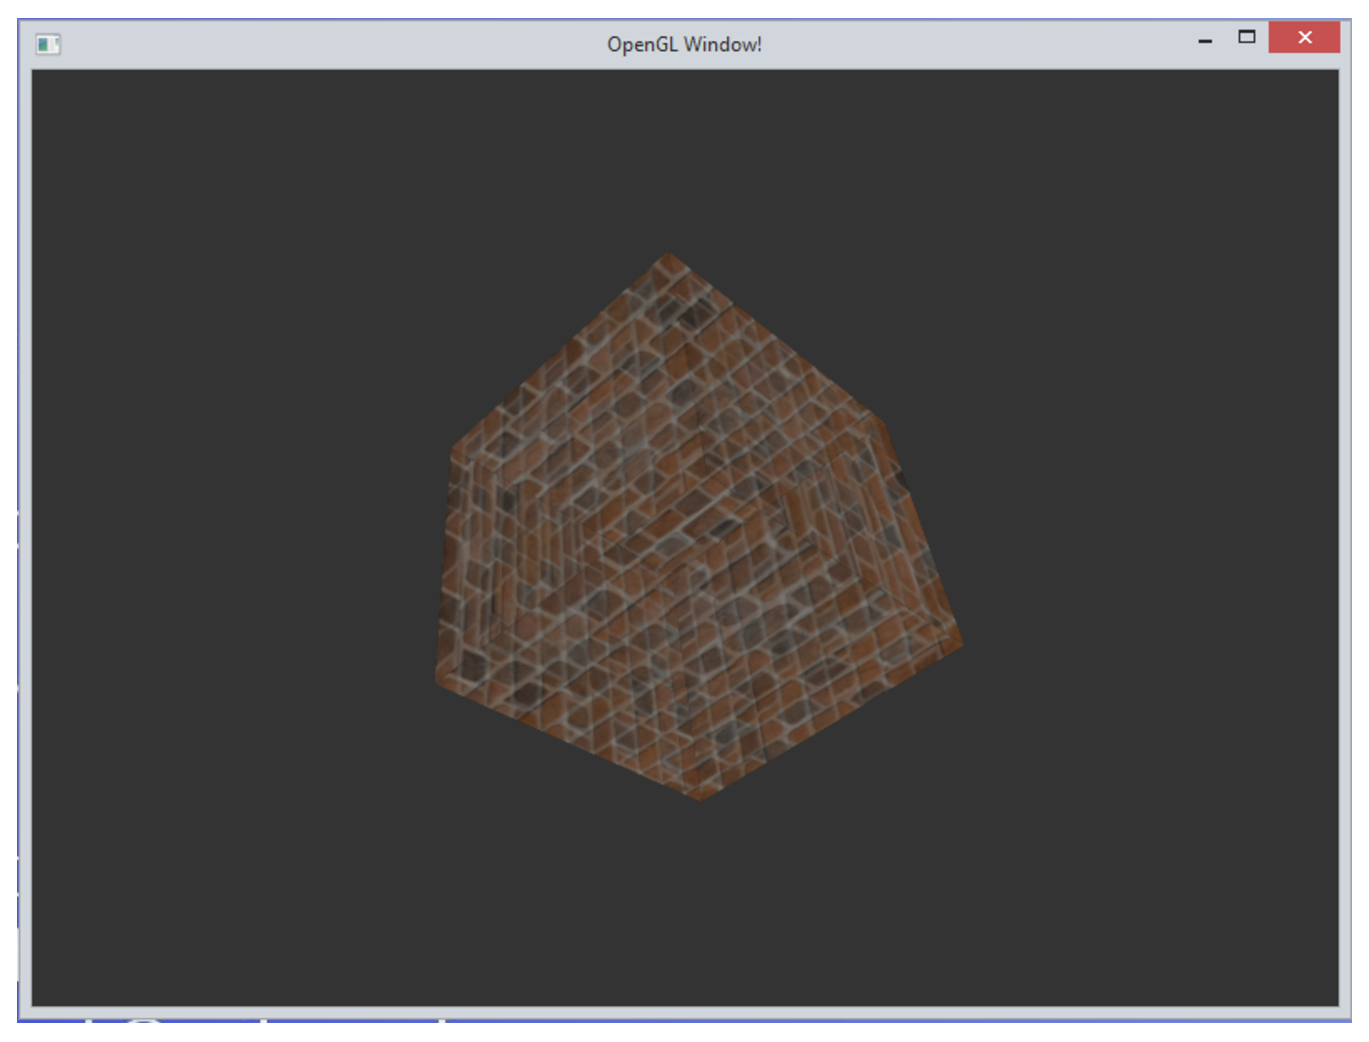
\includegraphics[width=0.50\textwidth]{graphics/screen_2.eps}
  \caption{Fading to transparent}
  \label{fig:screen_2}
\end{figure}

\begin{figure}[h!]
  \centering
  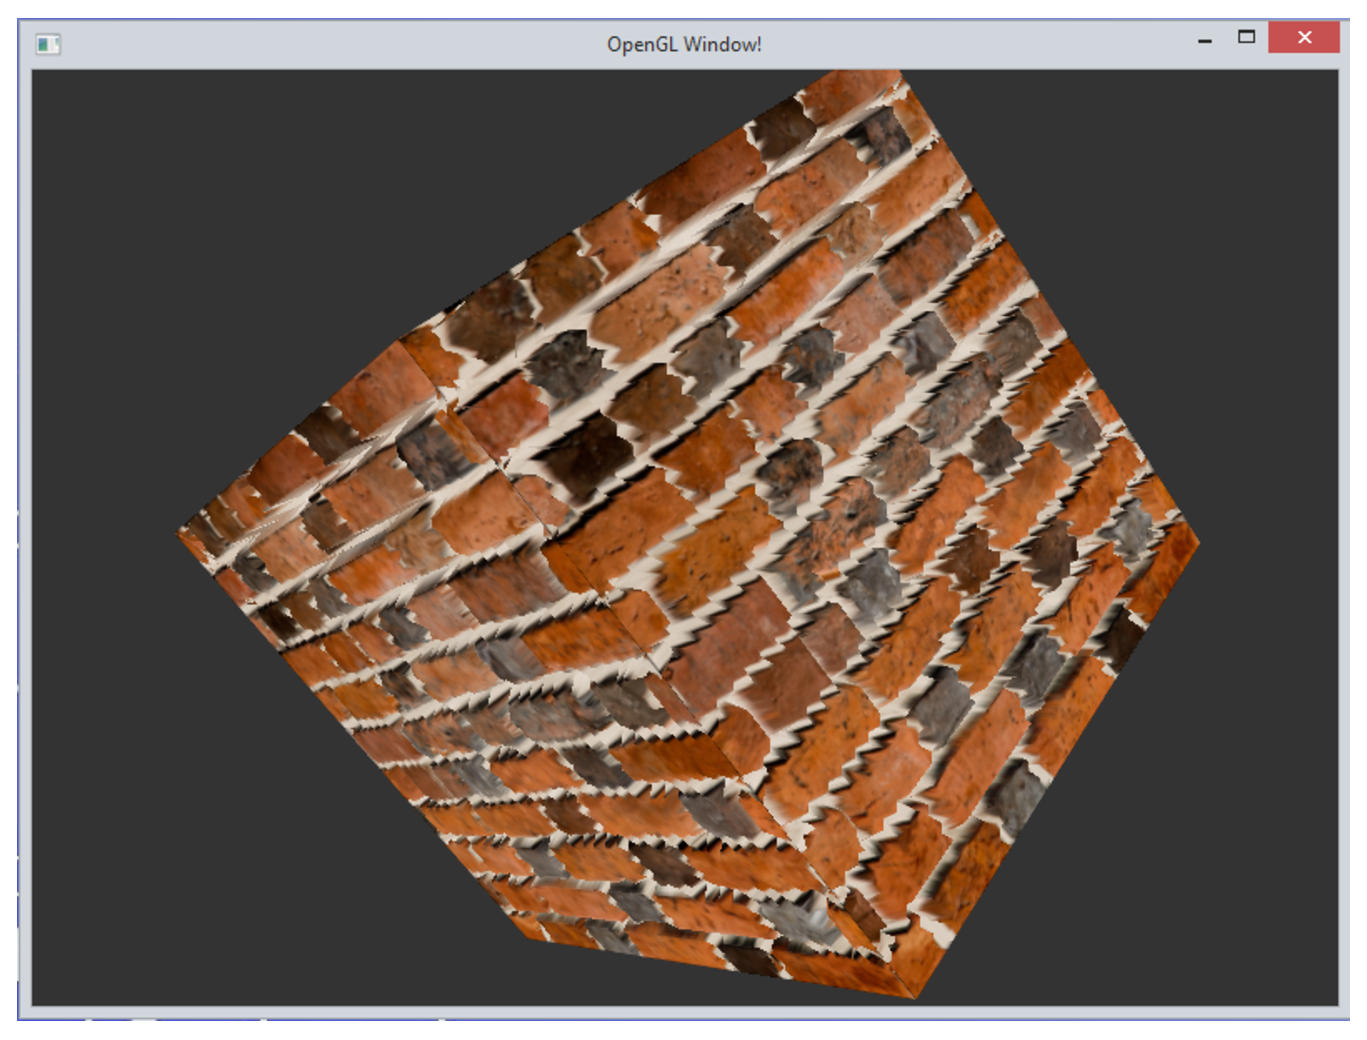
\includegraphics[width=0.50\textwidth]{graphics/screen_3.eps}
  \caption{Height map applied (reducing height of mortar)}
  \label{fig:screen_3}
\end{figure}

\begin{figure}[h!]
  \centering
  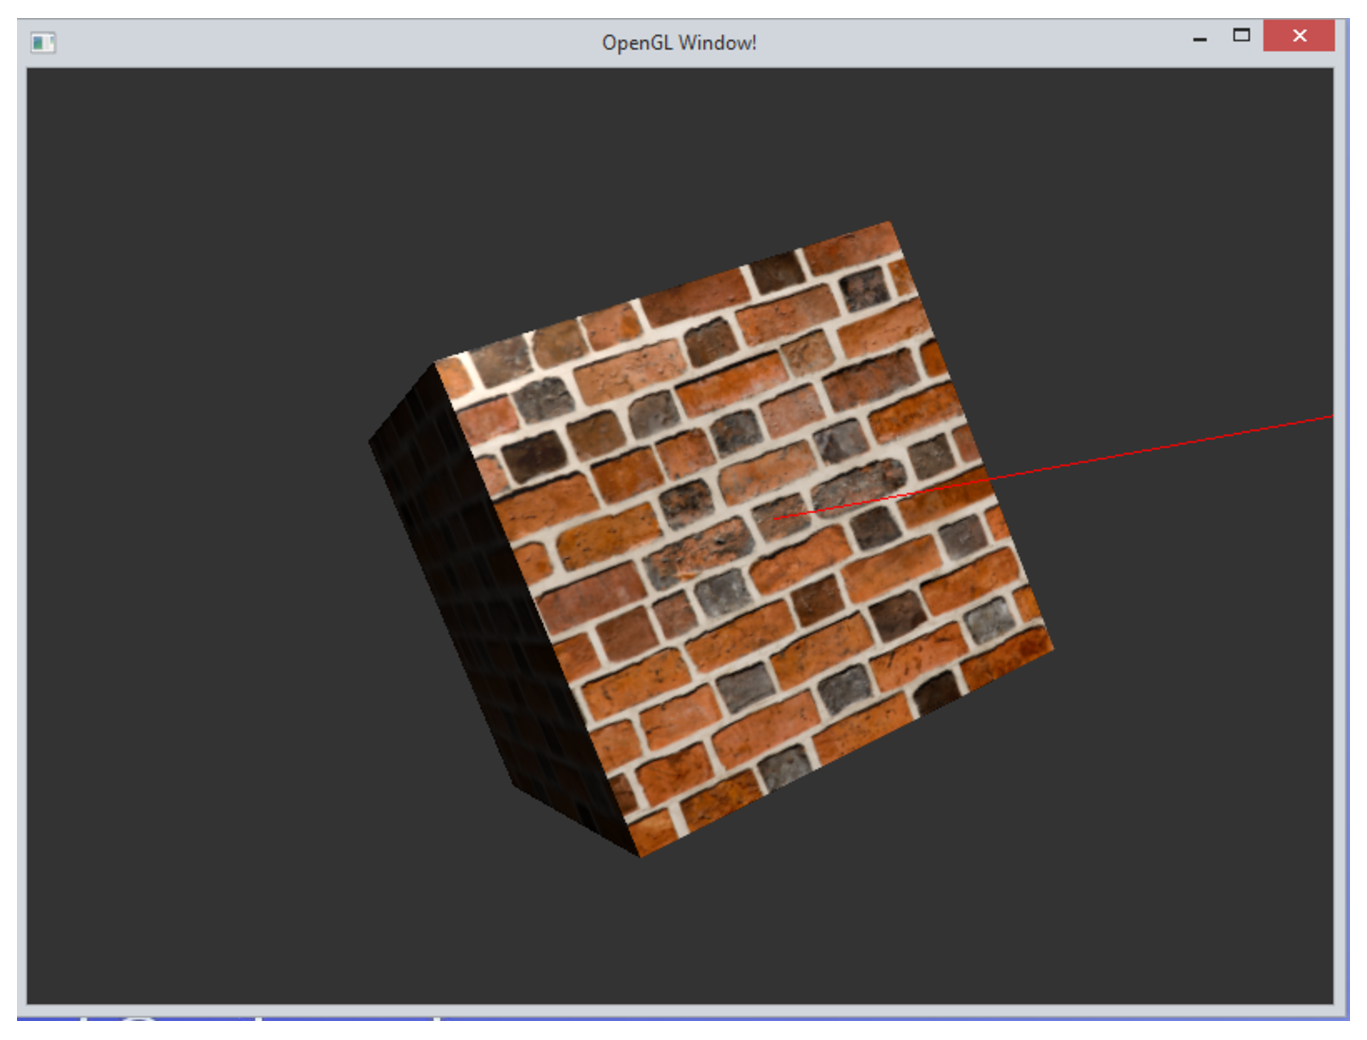
\includegraphics[width=0.50\textwidth]{graphics/screen_5.eps}
  \caption{Real time lighting (while light source from above)}
  \label{fig:screen_5}
\end{figure}

\begin{figure}[h!]
  \centering
  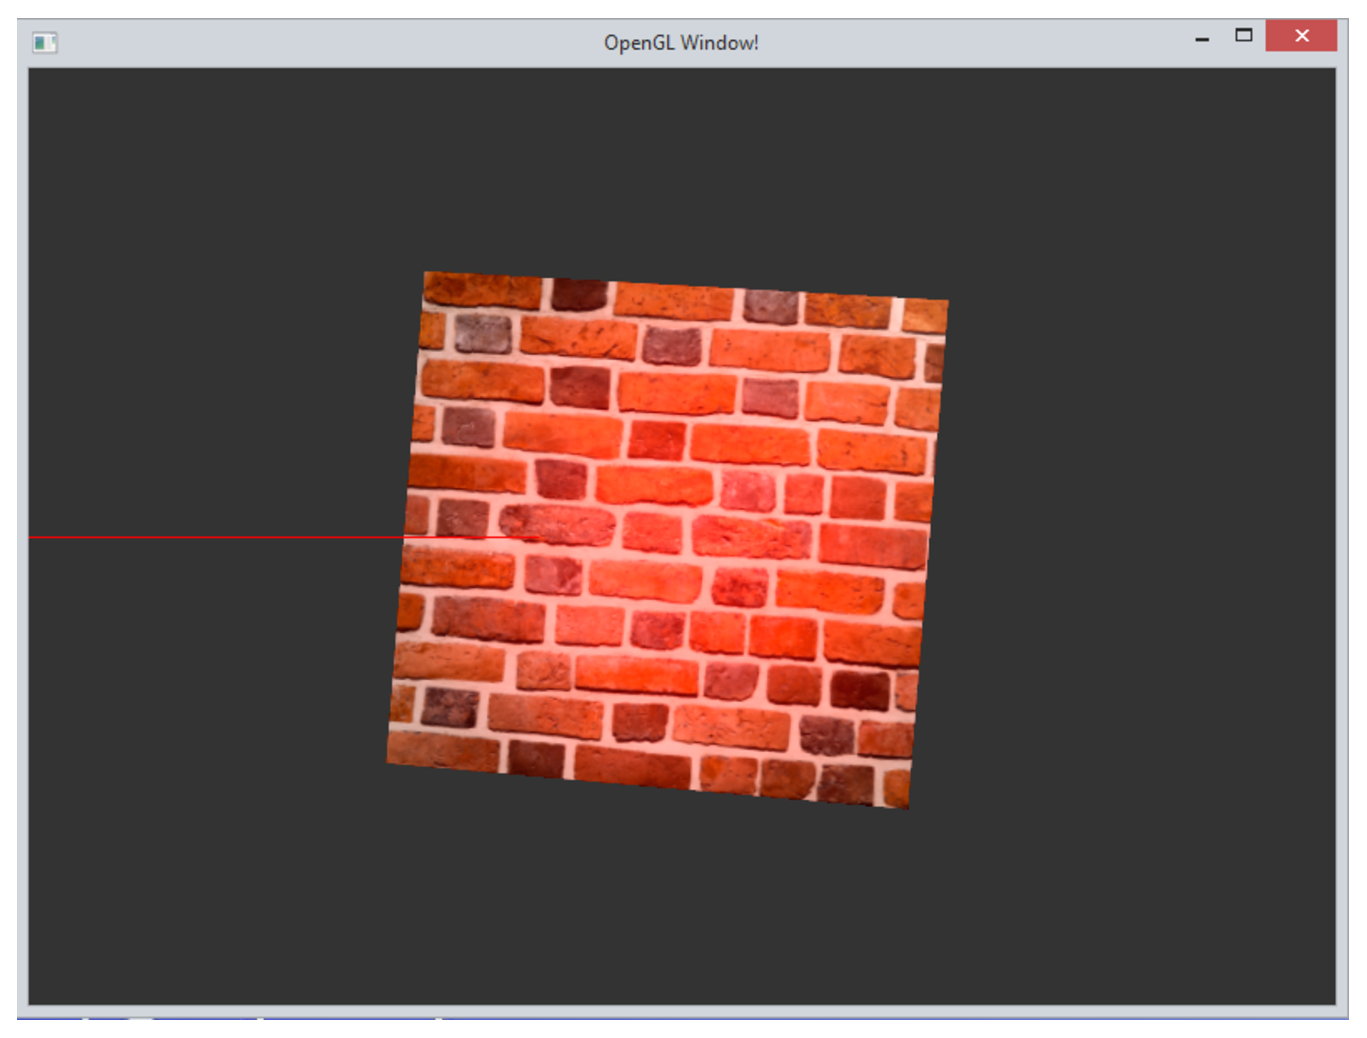
\includegraphics[width=0.50\textwidth]{graphics/screen_4.eps}
  \caption{Laser with two light sources (white from above, red form laser
           source)}
  \label{fig:screen_4}
\end{figure}

\begin{figure}[h!]
  \centering
  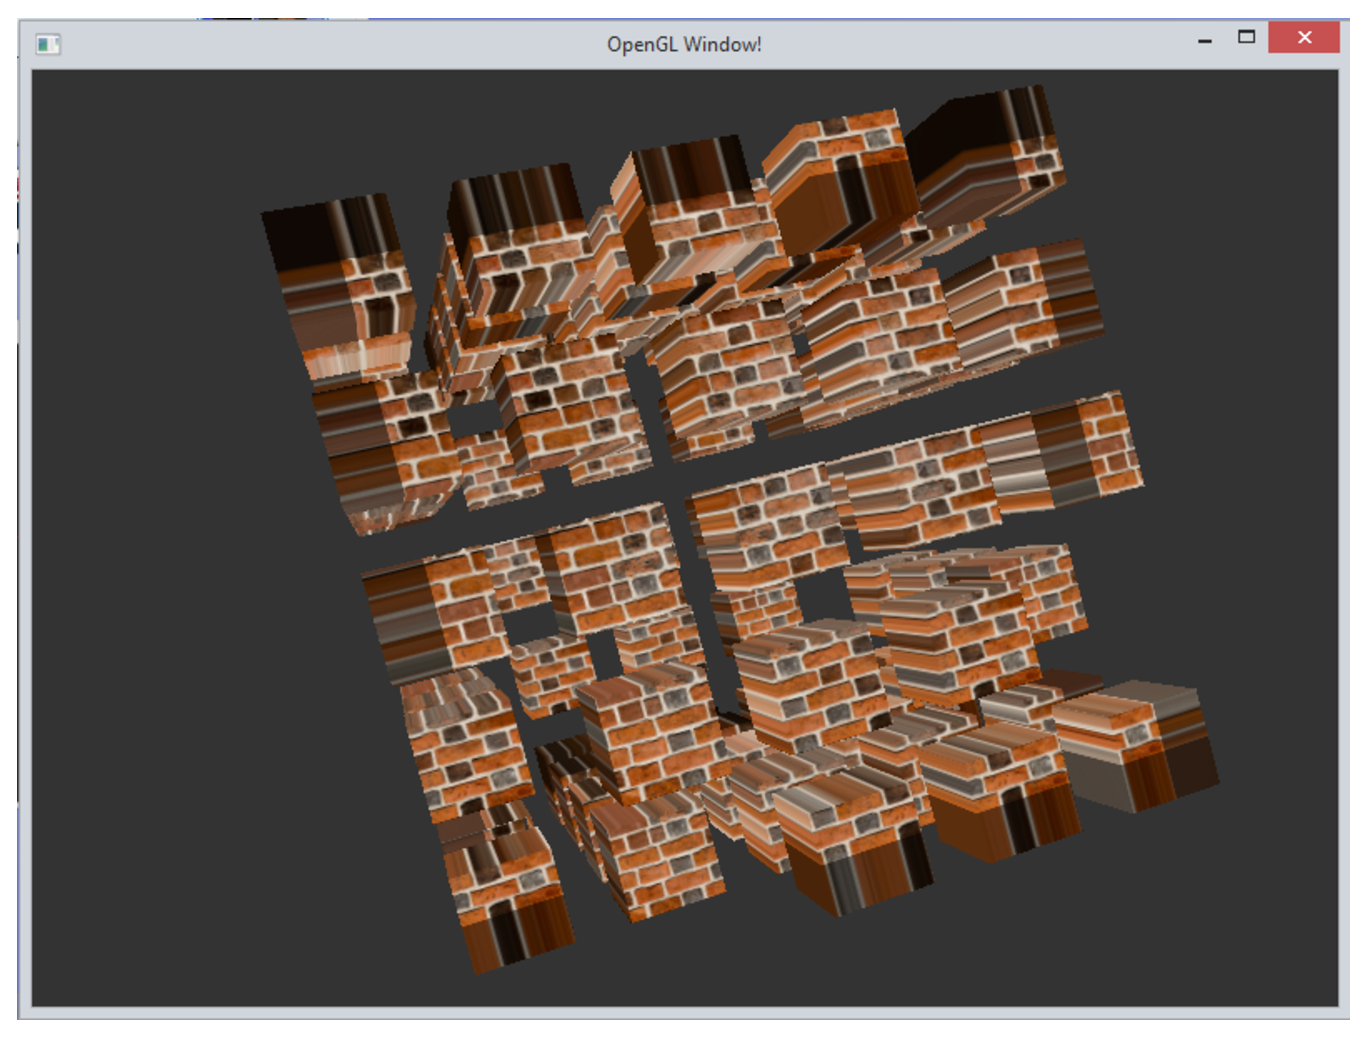
\includegraphics[width=0.50\textwidth]{graphics/screen_6.eps}
  \caption{Splitting cube into several smaller cubes}
  \label{fig:screen_6}
\end{figure}

\end{document}
